\documentclass[a4paper,titlepage]{article}

% use this when images are included
\usepackage{float}
\usepackage{graphicx}
\usepackage{subcaption}
\graphicspath{ {./images/} }

% use for lines of code
\usepackage{listings}

% use for links, also links list of contents
\usepackage{hyperref}


\title{Digital Pen}
\date{2021\\ June}
\author{Max-Felix Müller\\ \\ 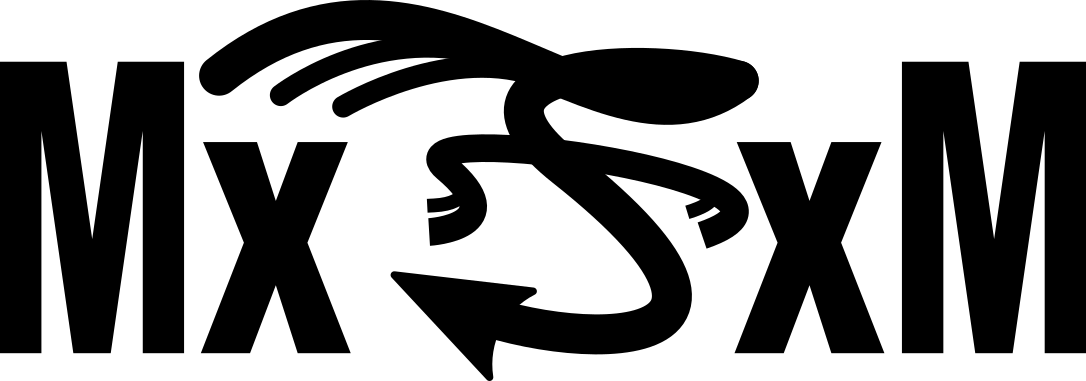
\includegraphics[width=\textwidth]{mxfxm.png}}

\begin{document}
\maketitle
\tableofcontents
\newpage
\listoffigures %delete if not necessary
\listoftables %delete if not necessary
\newpage

\section*{Abstract}

Using the Tiny Motion Trainer and an Arduino Nano 33 BLE Sense, a digital pen was created.

The digital pen can be used to draw letters into the air.
A neural network running on the microcontroller itself will predict which letter was drawn.
The accelerometer and gyroscope data is used for the prediction.

All letters can be detected with over 50\% certainty.
By modifying the example output of the Tiny Motion Trainer the model can be executed standalone.

An additionaly battery, charging and protection circuit could be added to make the pen truly wireless.

\newpage
\section{Inspiration}

What originally inspired this project was the video from Zack Freedman about his data glove.
The data glove is a glove with a motion sensor and a Teensy microcontroller.

It is nice that the glove also detects gestures, by measuring which fingers are extended.
That way the hand motion can be interpreted differently, for example to differentiate between a mouse and a keyboard interface.

However, the glove has to be worn and especially in hot summer days, this might not be preferable.

After receiving an advertisement of the Tiny Motion Trainer which can be used in conjuction with an Arduino Nano 33 BLE Sense to train a neural network to detect gestures, the project was started.

\section{Hardware}

The hardware for the project consists of a text marker and the Arduino Nano 33 BLE Sense.
The text marker can be cleaned once depleted and the Arduino will then fit inside.
Until then, the Arduino is just held on the side of the text marker using some rubber bands and tape to fix the power cable in place.

In a next step it would be possible to also fit a small lithium polymer battery inside the pen, along with a charging and boost circuit.
The pen could then connect via BLE and would be wireless.

\section{Tiny Motion Trainer Workflow}

The tiny motion trainer workflow is very similar to a "real" machine learning or deep learning workflow.

First the settings for the project are configured.
In this case, a small threshold is used to detect the start of the motion.
This is necessary, because the acceleration is measured and some letters do not have a high acceleration at the beginning.
100 samples are collected for each gesture, which supposedly gives about 1 second time, so 100 samples pre second.
After a letter is captured, the pen delays the next detection for 1 second to give the user some time to move his hand to a suitable starting position for the next motion.

The second step is to capture data.
Any number of labels (or at least more than 25) can be created.
For each label it is recommended to capture at least 20 samples.
The Arduino Nano connects via bluetooth directly to the browser.
This means that a browser with access to the bluetooth module of the laptop or PC has to be used, which would be Chrome or Edge (Edge is based on Chrome).

Then the model can be trained.
After training the model can directly in the browser be tested.

Once the results are satisfying, the model can be downloaded, even with an example code to directly compile and upload to the Arduino.
This code is then able to run without the bluetooth connection to a host PC.

\newpage
\section{Hello (World)}

Obviously the first word that comes to mind for a programmer is hello.
In german it is "Hallo", which consists of four different letters: H, a, l and o.

The intended use for a digital pen was something that would clip on to the back of a normal pen and that would digitalize the written letters.
After fixing the Arduino to a pen, letters were written on a piece of paper.

Normal handwriting draws very small letters, which becomes even more evident when looking at the signal amplitudes that were captured.
Even when drawing letters the size of a Din A5 page, the acceleration values were barely over the noise level.

\begin{figure}[H]
    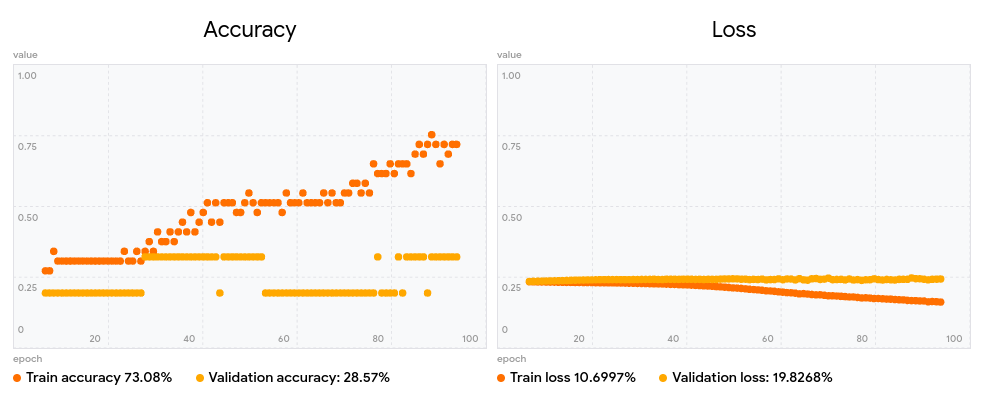
\includegraphics[width=\textwidth]{slow_training_start.png}
    \caption{No Accuracy Increase}
\end{figure}

When training the model with 10 samples for each letter, the resulting model was not really able to distinguish between the letters.
Due to this problem, the training also did not achieve high accuracy.
When training models on the mnist dataset, the accuracy rises very quickly in the beginning and the flattens out.
This is what was expected here also, but it did not happen.

\begin{figure}[H]
    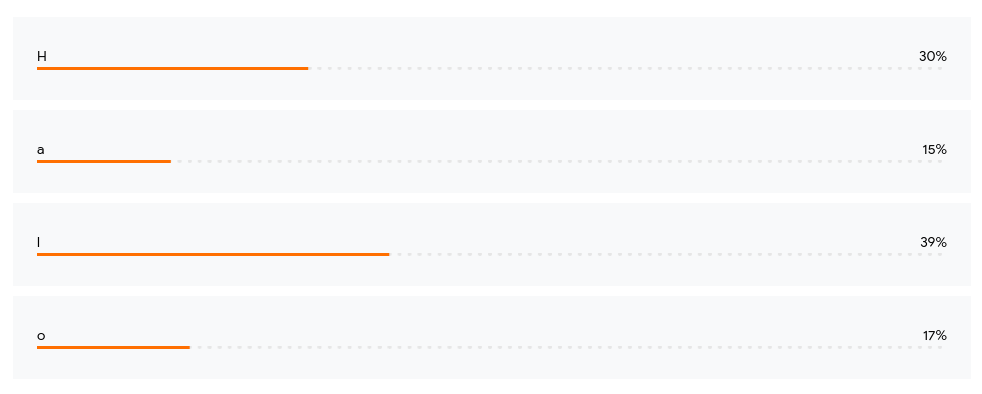
\includegraphics[width=\textwidth]{uncertain_results.png}
    \caption{Signal Level too Low}
\end{figure}

\subsection{Hello Iteration}

Since even the Din A5 sized letters were too small, the project idea was changed from detecting written letters to detecting letters that are drawn into the air.
The bigger letters also have larger acceleration at the corners or curves of the letter, thus better signals.

\begin{figure}[H]
    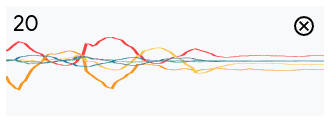
\includegraphics[width=\textwidth]{better_signal_A.png}
    \caption{Improved Signal for Letter 'A'}
\end{figure}

For better reproducibility the movement for each letter was noted on a piece of paper.
Dots represent corners or turning points in the gesture and the lines are the motions in between.
The numbers represent the order of the points.

The unique signals lead to training accuracy hitting 100\% after only 30 epochs.
This is technically bad, since it would mean that overfitting has occured.
However, the validation accuracy also reached 100\%.

\begin{figure}[H]
    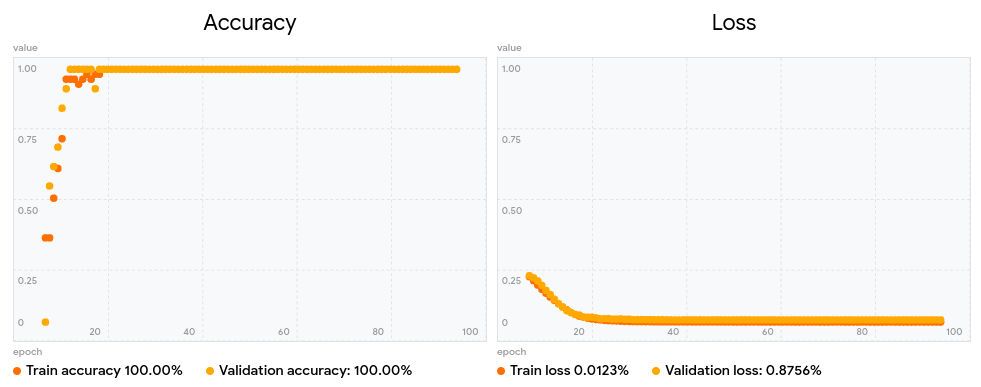
\includegraphics[width=\textwidth]{very_fast_training_reults_HALO.png}
    \caption{Easy Training}
\end{figure}

\newpage
This is possible, because the four signals of the letters have large variations.
Mistaking an 'l' (lower case L) for an 'o' for example is quite difficult.

There are a lot of letters that look very similar between upper and lower case.
For example lower case L and upper case i, or lower case o and upper case O.
Hence it was decided to go for upper case letters only.

The model was good enough to detect, capture and classify the letters 'H', 'A', 'L' and 'O'.

\begin{figure}[H]
    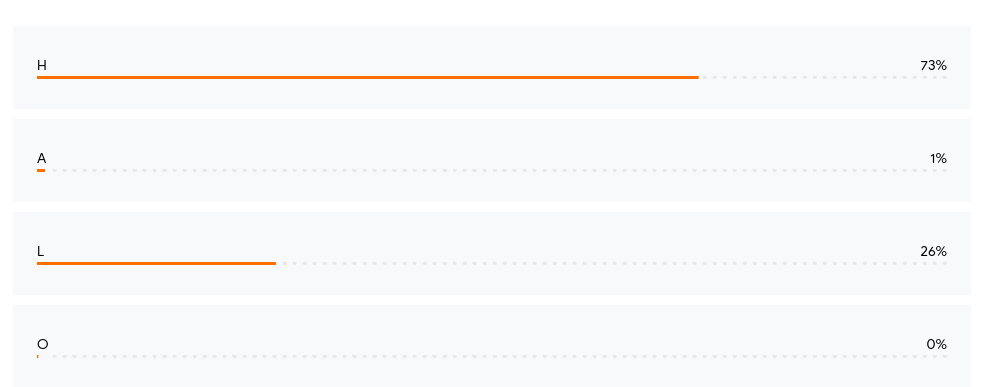
\includegraphics[width=\textwidth]{result_HALO.png}
    \caption{Result with 4 Letters 'H', 'A', 'L' and 'O'}
\end{figure}

\newpage
\section{Capturing the whole Alphabet}

More characters were added as labels.
This chapter is more of a lessons learned than anything else.

To have repeatable characters, the movements required were drawn on a piece of paper.
Later these could be adopted to achieve more unique signals.

A possible improvement would be to also capture some of the training data while standing up (and not sitting on a chair), because the hand movements vary slightly.

Sometimes the internet connection would cut out, losing some of the captured data.
It is important to save often.
This is no burden in this case, because the amount of data is very limited.

Large characters with high acceleration have stronger signals and thus help the model to achieve higher accuracy.

The more sample and classes (unique labels) that were added, the slower the training process became.

When restarting the training process on the Tiny Motion Trainer, the training starts over from zero.
It is better to start with a high number of epochs and stop early than having the training stop before hitting a good accuracy, just because the number of epochs was too small.
At first it looked like a good idea to run the training for 260 epochs (26 characters times 10), but later it was discovered, that 500 is a better number.

The accuracy was in the range of 89\% at first.
With 1 of 26 being about 0.04 and 3 out of 26 about 0.11 this would mean that 3 characters could not be recognized or distinguished in the training.

The training was suspiciously slow on the chromebook I used at first.
As it turns out, Tiny Motion Trainer does not run the training on some Google server, but on the local machine instead.
While running it on a better equipped desktop computer, it seems to even make use of the installed NVIDIA GPU, making training about 100 times faster.
Instead of hours the training only took minutes.
The fast loop time is essential for fast iterations and thus fast improvement.

The whole project with all sampmles is saved as one .json file which enables moving the whole project between machines for data capture and training.
This was necessary, because the desktop PC does not have BLE to connect to the Arduino for data capture.

After failing to recognize some characters, a closer look at the data was in order.
It became obvious, that the "bad" characters do have very different samples.
This is due to the threshold for the detection of the start of the movement.
While looking through the captured samples, this was the case more often than I'd like to admit.

\begin{figure}[H]
    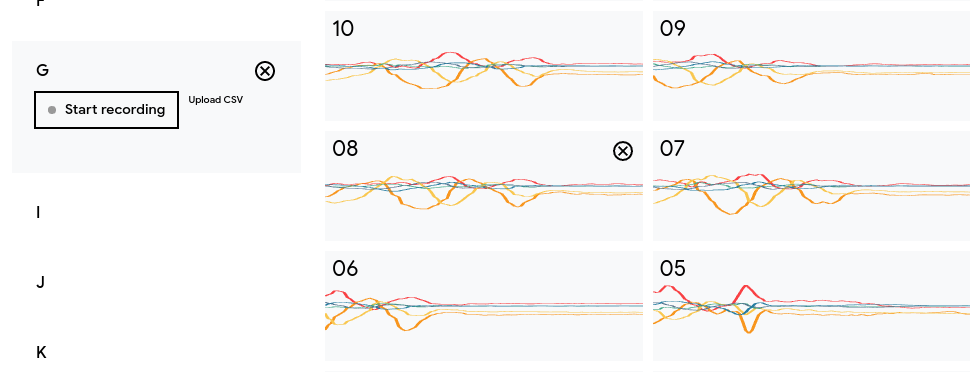
\includegraphics[width=\textwidth]{different_samples_not_good.png}
    \caption{Different G Samples due to Detection Threshold}
\end{figure}

The number and position of the peaks in the sample should be similar.
This also means that the movement was done uniformly.
There are no faster or slower parts to it.

This is even more important when looking at the model used for recognition.
Instead of some kind of LSTM, a typical convolutional neural network is used.
Due to the memory and speed constrains of the microcontroller, this makes sense.
With a task that would benefit of time data, or rather the different parts of the movement being recognized one after the other, it is not ideal.

The Arduino also captures gyroscope data alongside the acceleration.
Some characters thus rely on a turning motion of the wrist.
Even small variation in the movement decides between no detection at all and more than 90\%.

\begin{figure}[H]
    \begin{subfigure}[b]{\linewidth}
        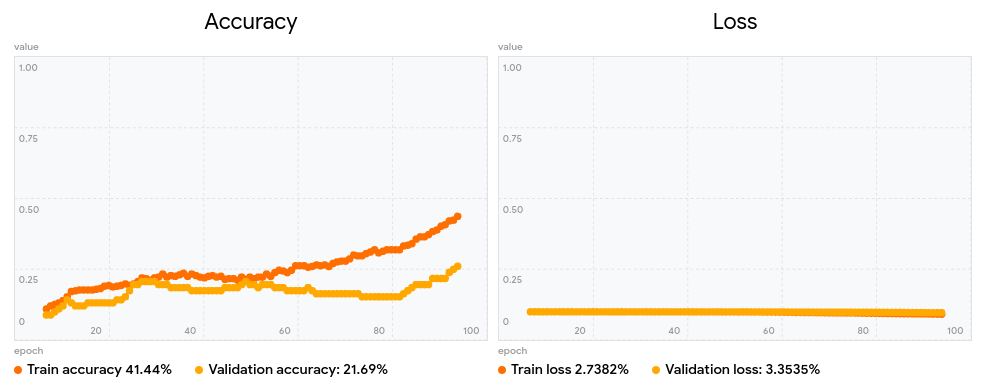
\includegraphics[width=\linewidth]{train_1.png}
        \caption{Starting with Bad Samples}
    \end{subfigure}
    \begin{subfigure}[b]{\linewidth}
        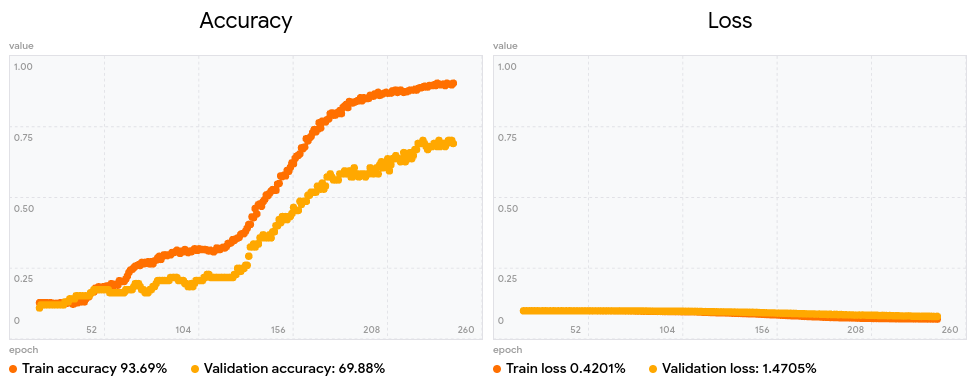
\includegraphics[width=\linewidth]{train_2.png}
        \caption{Better Samples}
    \end{subfigure}
    \begin{subfigure}[b]{\linewidth}
        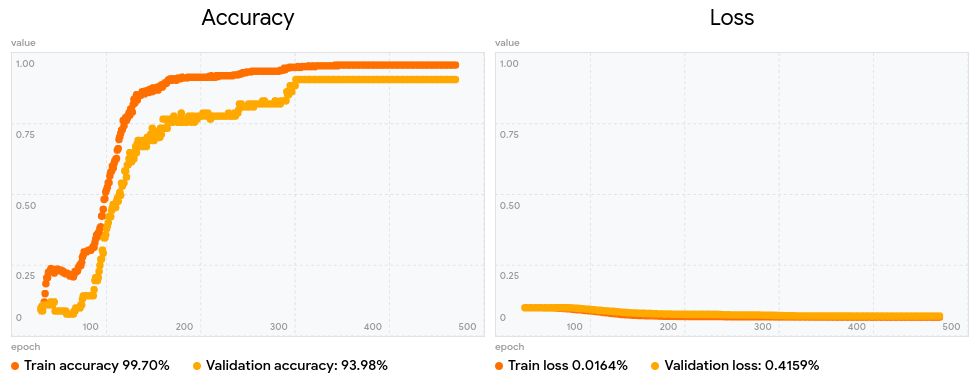
\includegraphics[width=\linewidth]{train_3.png}
        \caption{Good Samples and Longer Training}
    \end{subfigure}
    \caption{Influence of Sample Quality}
\end{figure}

All in all it took 10 iterations to get a working model.

\newpage
\subsection{New Character Movements}

These characters were re-captured, because they could not be distinguished by the model:

D was changed to lower case character, because it was too similar to B.

F was too similar to E at the beginning.
It was changed to a lower case f, in order to have a more unique movement with the arc on top.

G showed very bad accuracy due to its similarity to O, C and Q.
It was changed to lower case.

J was not classified to any letter, not even a wrong one.
All classes had a small percentage of possibility.
This is wired, because there is no similar character.

K movement was improved by making it closer to a lower case k (at least for me).

L was captured once more, to have a more pronounced change in direction between the horizontal and the vertical part.

S was not recognized at first.
The movement was changed to represent more of an 8 than the S, to have stronger and fuller arcs / circles.

X movement had to be captured again.
The pen seems to have been turned slightly when capturing the original samples.
When the pen was held at an angle the classigication was very good, while it would not recognize the X at all when the pen was hold at the same angle as for the other characters.

\newpage
\section{Example Code}

The Tiny Motion Trainer allows to download the model with an Arduino example code to directly compile.
This is a very nice feature to get started quickly.
The code can easily be changed to fit specific needs.

\subsection{Understanding the Example}

The model is packed as a large byte array into its own header file.
There is not too much to understand.
This will be different for every project.

The rest of the code is a "one size fits all" kind of solution.

There is one section that is project specific.
The settings are entered here, threshold, capture delay and the number of samples.
There is also an array that holds the label for each output of the neural network.

\begin{lstlisting}
// Values from Tiny Motion Trainer
#define MOTION_THRESHOLD 0.1
#define CAPTURE_DELAY 1000 // This is now in milliseconds
#define NUM_SAMPLES 100

// Array to map gesture index to a name
const char *GESTURES[] = {
    "H", "A", "L", "O", "B", "C", "D", "E", "F", "G", ...
};
\end{lstlisting}

After initializing the inertial measurement unit, the sample rate is read and displayed.
This will become important later on.
If the initialization fails, the code loops forever and does not continue.

\begin{lstlisting}
// Initialize IMU sensors
if (!IMU.begin()) {
    Serial.println("Failed to initialize IMU!");
    while (1);
}

// Print out the samples rates of the IMUs
Serial.print("Accelerometer sample rate: ");
Serial.print(IMU.accelerationSampleRate());
Serial.println(" Hz");
Serial.print("Gyroscope sample rate: ");
Serial.print(IMU.gyroscopeSampleRate());
Serial.println(" Hz");
\end{lstlisting}

The memory for the model is allocated and pointers are initialized to point to the first layer, as input, and the last layer to retrieve the output.

\begin{lstlisting}
// Allocate memory for the model's input and output tensors
tflInterpreter->AllocateTensors();

// Get pointers for the model's input and output tensors
tflInputTensor = tflInterpreter->input(0);
tflOutputTensor = tflInterpreter->output(0);
\end{lstlisting}

The main loop reads acceleration and gyroscope data until the threshold is met.
Then the loop breaks and the sampling starts.

\begin{lstlisting}
// Above the threshold?
if (average >= MOTION_THRESHOLD) {
    isCapturing = true;
    skip_next_sample = false;
    numSamplesRead = 0;
    break;
}
\end{lstlisting}

Sampling will continue until the required number of samples was captured.

\begin{lstlisting}
// Do we have the samples we need?
if (numSamplesRead == NUM_SAMPLES) {
\end{lstlisting}

The samples are written directly to the input pointer of the model.
An offset is added between each sample.
The values are also normalized before they are written to the input.
Having values in the range of -1 to 1 helps the training of the neural network.
This normalization is also done for the initial data capturing befor training.
If it were done only here, the network would not work correctly.
In this case the gyroscope sampels would be too high in comparison, because they reach from -2000 to 2000 while the acceleration is only within -4 and 4.

\begin{lstlisting}
// Normalize the IMU data between -1 to 1 and store in the model's
// input tensor. Accelerometer data ranges between -4 and 4,
// gyroscope data ranges between -2000 and 2000
tflInputTensor->data.f[numSamplesRead * 6 + 0] = aX / 4.0;
tflInputTensor->data.f[numSamplesRead * 6 + 1] = aY / 4.0;
tflInputTensor->data.f[numSamplesRead * 6 + 2] = aZ / 4.0;
tflInputTensor->data.f[numSamplesRead * 6 + 3] = gX / 2000.0;
tflInputTensor->data.f[numSamplesRead * 6 + 4] = gY / 2000.0;
tflInputTensor->data.f[numSamplesRead * 6 + 5] = gZ / 2000.0;
\end{lstlisting}

Inference is run by calling one single function.
The reults is checked afterwards, for errors during execution.

\begin{lstlisting}
// Run inference
TfLiteStatus invokeStatus = tflInterpreter->Invoke();
\end{lstlisting}

Then a loop can run over the results, looking for the highest probability sample.

\begin{lstlisting}
for (int i = 0; i < NUM_GESTURES; i++) {
    float _value = tflOutputTensor->data.f[i];
    if(_value > maxValue){
        maxValue = _value;
        maxIndex = i;
    }
}
\end{lstlisting}

\subsection{Fixes}

\begin{lstlisting}
\end{lstlisting}

\begin{lstlisting}
\end{lstlisting}

\begin{lstlisting}
\end{lstlisting}

\begin{lstlisting}
\end{lstlisting}

\newpage
\section{Links}

Ressources used for an in this project: \\

The video from Zack Freedman \\
\href{https://www.youtube.com/watch?v=6raRftH9yxM}{https://www.youtube.com/watch?v=6raRftH9yxM} \\

Tiny Motion Trainer \\
\href{https://experiments.withgoogle.com/tiny-motion-trainer}{https://experiments.withgoogle.com/tiny-motion-trainer} \\

\end{document}
